\section{Data scaling vs.\ the aleatoric floor}
\label{sec:data_scaling}

This section complements the pre-registered questions in §\ref{sec:ablations}: we ask how quickly error decreases when the training fraction of \scthree{} is increased, and whether extrapolated learning curves ever intersect the split-specific aleatoric RMSE floors derived from duplicate laboratory triples.

\subsection{Split-specific aleatoric RMSE floors}
\label{sec:scaling_floors_sub}

For each benchmark split $s$ (Train, Eval, OOD, Gold-tier analogue \texttt{sc3\_gold}), we estimate an RMSE-comparable aleatoric floor from duplicate $(\text{solute},\text{solvent},\mathrm{round}(T,0))$ triples: observations within the same triple $g$ are treated as repeated draws of the same underlying label.
Let $\bar{y}_g$ be the mean label in group $g$, $n_g$ the number of observations in $g$, and $N=\sum_g n_g$ the total count of observations participating in duplicate groups on split $s$.
We define
\begin{equation}
  (\epsA^{(s)})^2 \;=\; \frac{1}{N}\sum_{g}\sum_{i\in g}\bigl(y_i-\bar{y}_g\bigr)^2 .
  \label{eq:eps_split}
\end{equation}
Values are reported in Table~\ref{tab:scaling_floors}; they serve as split-specific references when interpreting the asymptotes of fitted scaling curves below.

\subsection{Empirical scaling curves}
\label{sec:scaling_curves_sub}

We subsample the training pool at fractions $\{0.05,0.10,0.20,0.40,0.60,0.80,1.00\}$ (stratified by solvent) and retrain representative models---\textsc{LightGBM} on RDKit descriptors and several \textsc{FastProp} MLP widths---holding evaluation splits fixed.
Figure~\ref{fig:data_scaling_curves} summarises test RMSE vs.\ training-set size; Figure~\ref{fig:data_scaling_train_vs_val} decomposes train vs.\ test behaviour; Figure~\ref{fig:data_scaling_lawfits} overlays saturating power-law fits $\mathrm{RMSE}(N)\approx a N^{-b}+c$.

\begin{figure}[t]
  \centering
  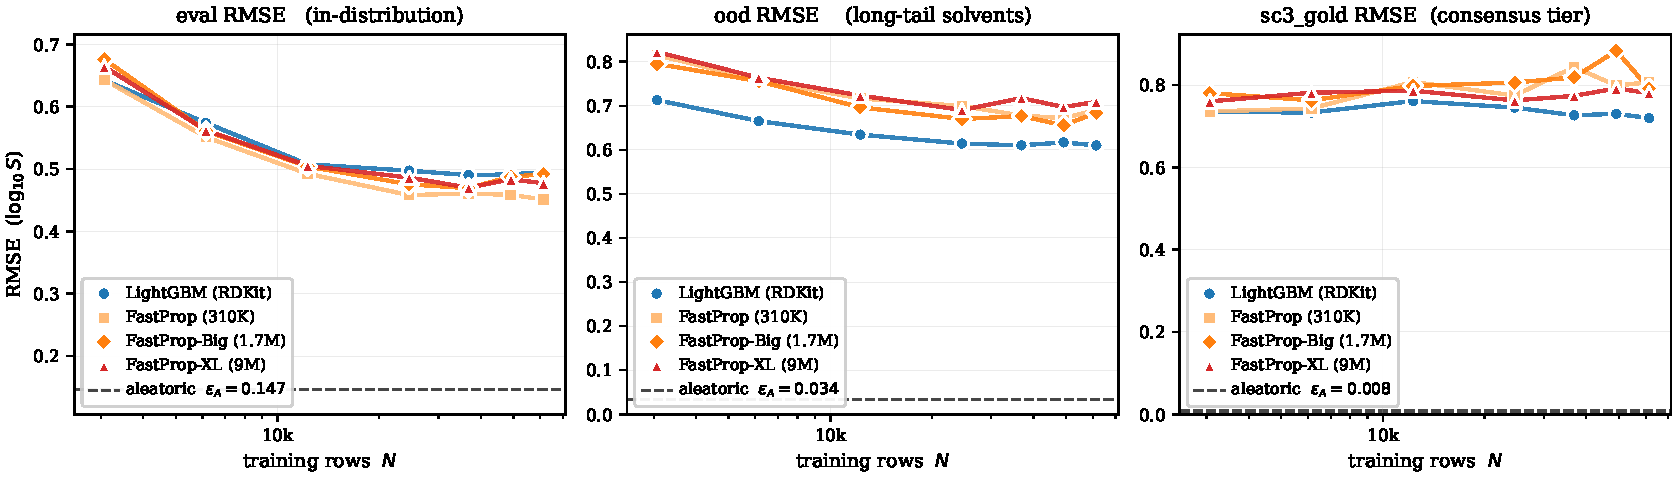
\includegraphics[width=\linewidth]{figures/fig_data_scaling_curves.pdf}
  \caption{Test RMSE vs.\ training-set fraction for representative models (seven fractions $\times$ fixed seeds).}
  \label{fig:data_scaling_curves}
\end{figure}

\begin{figure}[t]
  \centering
  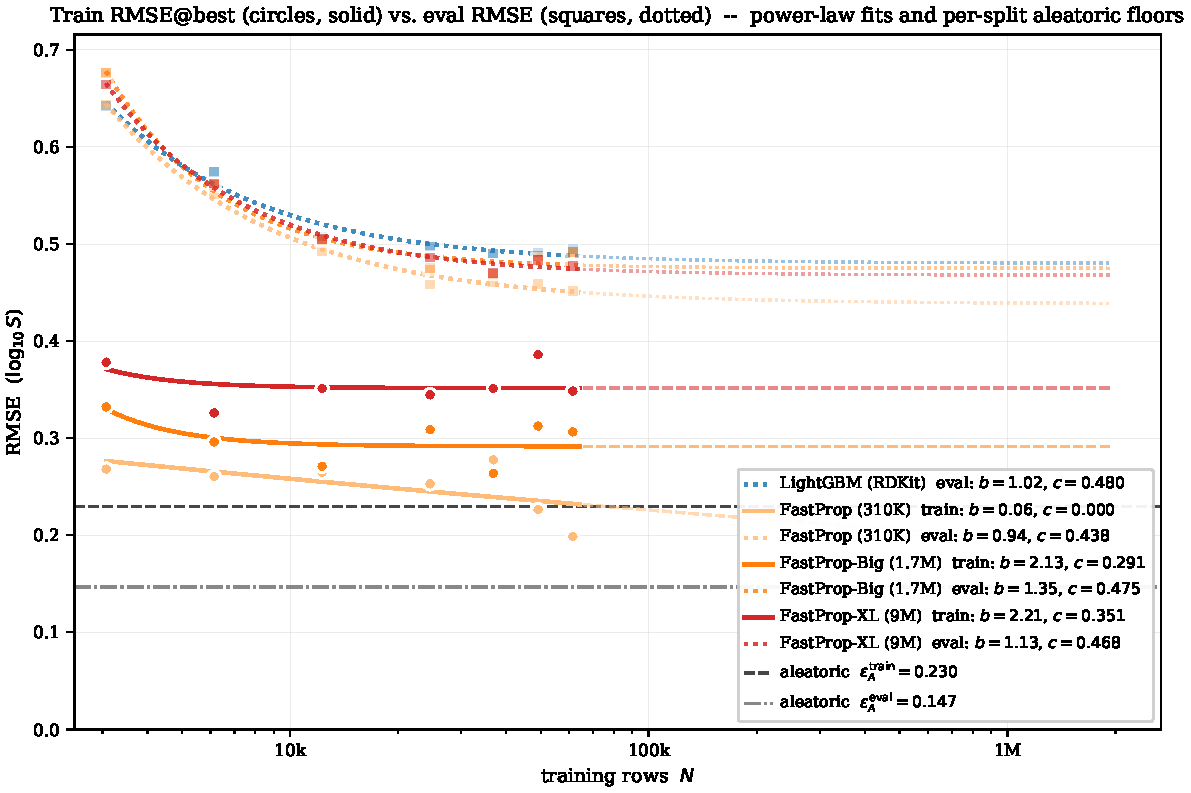
\includegraphics[width=\linewidth]{figures/fig_data_scaling_train_vs_val.pdf}
  \caption{Train vs.\ test RMSE across fractions (diagnostic for overfitting vs.\ noise floor).}
  \label{fig:data_scaling_train_vs_val}
\end{figure}

\begin{figure}[t]
  \centering
  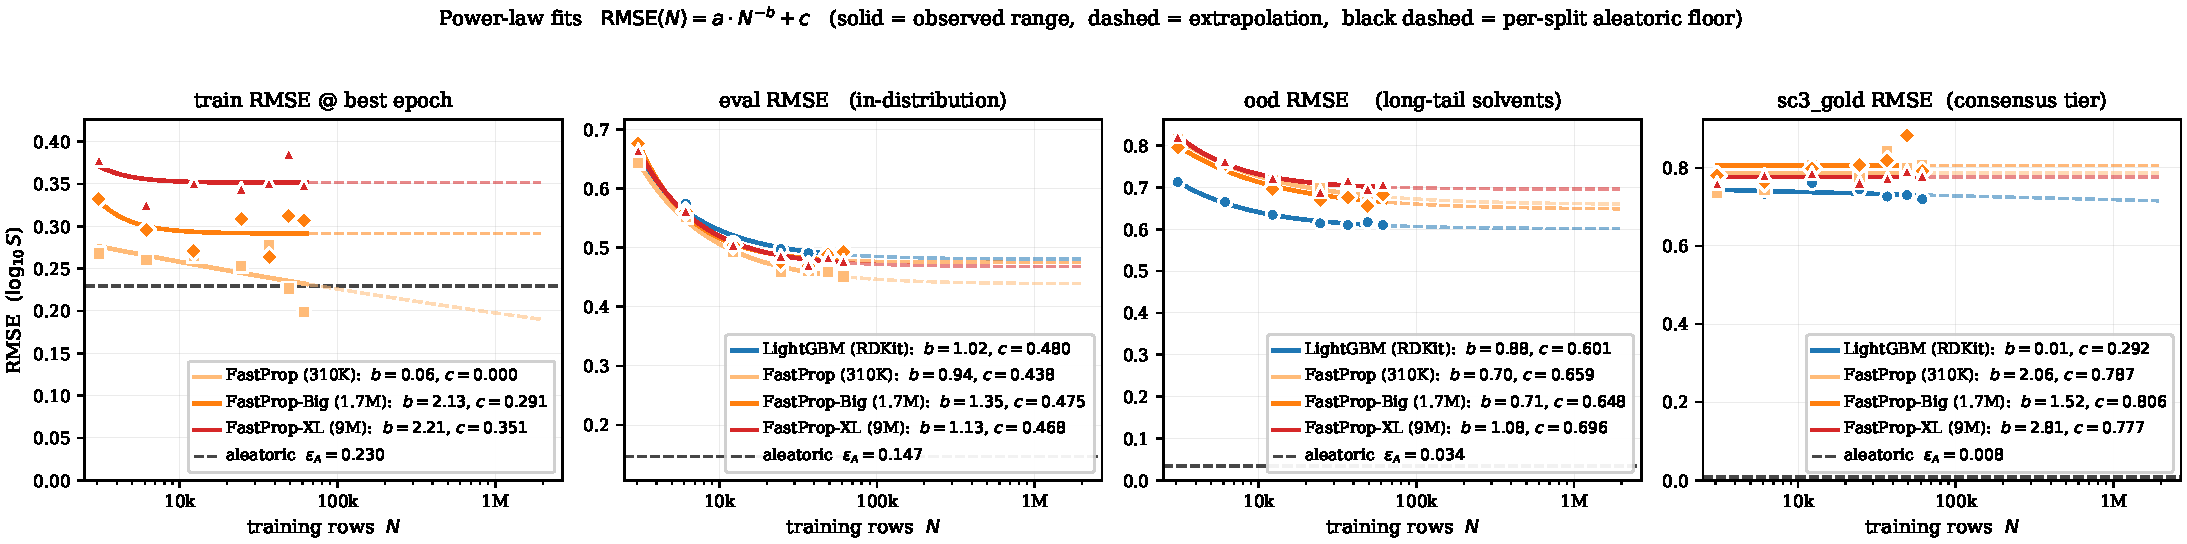
\includegraphics[width=\linewidth]{figures/fig_data_scaling_lawfits.pdf}
  \caption{Saturating power-law fits to the empirical scaling curves (same fits as Table~\ref{tab:scaling_fits}).}
  \label{fig:data_scaling_lawfits}
\end{figure}

\begin{table}[h]
\centering\small
\caption{Per-split aleatoric RMSE floors $\epsA$ from
  Eq.~\ref{eq:eps_split}, computed on duplicate
  $(\text{solute}, \text{solvent}, \mathrm{round}(T,0))$ triples within
  each split.  $n_{\text{trip}}$ is the number of duplicate triples;
  $n_{\text{obs}}$ is the total number of observations participating
  in those triples (each contributes one residual against its group
  mean).  Median per-triple std and the $90$th percentile capture the
  shape of the within-triple disagreement distribution: medians are
  sub-millimolar everywhere, and the heavy right tail is what drives
  $\epsA$ above the median.  $\epsA$ is RMSE-comparable to the model
  RMSE reported on the same split.}
\label{tab:scaling_floors}
\begin{tabular}{@{}lrrrrrr@{}}
\toprule
split & $n_{\text{trip}}$ & $n_{\text{obs}}$ & $\epsA$ (RMSE) & MAE floor & $P_{50}$ & $P_{90}$ \\
\midrule
\texttt{train}    & \numval{905} & \numval{1\,839} & \numval{0.230} & \numval{0.074} & \numval{0.005} & \numval{0.430} \\
\texttt{eval}     & \numval{101} & \numval{202}    & \numval{0.147} & \numval{0.038} & \numval{0.005} & \numval{0.026} \\
\texttt{ood}      & \numval{83}  & \numval{166}    & \numval{0.034} & \numval{0.009} & \numval{0.002} & \numval{0.024} \\
\texttt{sc3\_gold} & \numval{490} & \numval{988}   & \numval{0.008} & \numval{0.004} & \numval{0.002} & \numval{0.012} \\
\bottomrule
\end{tabular}
\end{table}


\subsection{Power-law asymptotes}
\label{sec:scaling_powerlaw}

Table~\ref{tab:scaling_fits} lists least-squares fits of $\mathrm{RMSE}(N)=a N^{-b}+c$ on the seven-point scaling curves.
The intercept $c$ is interpreted as the best RMSE achievable at infinite training data \emph{for the fixed representation and architecture}; it should be compared to $\epsA^{(s)}$ from Eq.~\ref{eq:eps_split}, not to the global inter-laboratory $\epsA$ of §\ref{sec:epsA}.

\begin{table}[h]
\centering\small
\caption{Power-law fits $\mathrm{RMSE}(N) = a \cdot N^{-b} + c$ per
  (model, evaluation split), plus the train-side fit (only available for
  the deep models; LightGBM does not save a per-fraction train-RMSE
  diagnostic).  $b$ is the scaling exponent (larger = more bang per
  data row).  $c$ is the model's irreducible asymptote (smaller =
  better in the limit of infinite data).  $R^{2}$ is the coefficient
  of determination of the fit on the seven $(N, \mathrm{RMSE})$ points.
  The asymptote $c$ is the column to read for Q4: it is the model's
  best achievable RMSE on this split, given infinite data and the same
  representation.}
\label{tab:scaling_fits}
\begin{tabular}{@{}llrrrr@{}}
\toprule
model              & split           & $a$           & $b$    & $c$            & $R^{2}$ \\
\midrule
\textsc{LightGBM}  & \texttt{eval}    & \numval{588.43} & \numval{1.02} & \numval{0.480} & \numval{0.98} \\
\textsc{LightGBM}  & \texttt{ood}     & \numval{131.38} & \numval{0.88} & \numval{0.601} & \numval{0.99} \\
\textsc{LightGBM}  & \texttt{sc3\_gold}& \numval{0.49}   & \numval{0.01} & \numval{0.292} & \numval{0.13} \\
\midrule
\textsc{FastProp}  & \texttt{eval}    & \numval{382.15} & \numval{0.94} & \numval{0.438} & \numval{0.99} \\
\textsc{FastProp}  & \texttt{ood}     & \numval{45.07}  & \numval{0.70} & \numval{0.659} & \numval{0.98} \\
\textsc{FastProp}  & \texttt{sc3\_gold}& \numval{$\sim$0}& \numval{2.06} & \numval{0.787} & --- \\
\textsc{FastProp}  & \texttt{train}   & \numval{0.44}   & \numval{0.06} & \numval{$\sim 0$} & \numval{0.36} \\
\midrule
\textsc{FastProp-Big}& \texttt{eval}  & \numval{10\,262.47}& \numval{1.35}& \numval{0.475} & \numval{0.98} \\
\textsc{FastProp-Big}& \texttt{ood}   & \numval{47.26}  & \numval{0.71} & \numval{0.648} & \numval{0.94} \\
\textsc{FastProp-Big}& \texttt{sc3\_gold}& \numval{$\sim$0}& \numval{1.52}& \numval{0.806} & --- \\
\textsc{FastProp-Big}& \texttt{train} & \numval{$10^{6}$}& \numval{2.13}& \numval{0.291} & \numval{0.35} \\
\midrule
\textsc{FastProp-XL} & \texttt{eval}  & \numval{1\,740.30}& \numval{1.13}& \numval{0.468} & \numval{0.99} \\
\textsc{FastProp-XL} & \texttt{ood}   & \numval{734.60} & \numval{1.08} & \numval{0.696} & \numval{0.95} \\
\textsc{FastProp-XL} & \texttt{sc3\_gold}& \numval{0.83}& \numval{2.81} & \numval{0.777} & --- \\
\textsc{FastProp-XL} & \texttt{train} & \numval{$10^{6}$}& \numval{2.21}& \numval{0.351} & \numval{0.13} \\
\bottomrule
\end{tabular}
\end{table}


\subsection{Extrapolated crossing with the aleatoric floor}
\label{sec:scaling_q4}

Given a fitted asymptote $c$, split floor $\epsA^{(s)}$, and tolerance $\delta=0.05$~log~S, the hypothetical training-set size at which the power-law model would match the aleatoric reference satisfies
\begin{equation}
  a\,(N^\star_{\epsA})^{-b} + c \;\le\; \epsA^{(s)} + \delta .
  \label{eq:nstar}
\end{equation}
Whenever $c>\epsA^{(s)}+\delta$, no finite $N^\star_{\epsA}$ exists within the saturating model---Table~\ref{tab:scaling_extrapolation} marks this case as $\infty$.
We additionally report $N^\star_{95}$, the size at which RMSE reaches within $5$\% of the model's \emph{own} asymptote $c$, as a data-efficiency summary independent of $\epsA^{(s)}$.

\begin{table}[h]
\centering\small
\caption{Q4 extrapolation table.  For every (model, evaluation split)
  pair we report the asymptote $c$ from
  Table~\ref{tab:scaling_fits}, the per-split aleatoric floor $\epsA$
  from Table~\ref{tab:scaling_floors}, the gap $\Delta = c - \epsA$,
  the training-set size $N^{\star}_{95}$ at which RMSE comes within
  $5\%$ of the model's own asymptote (a moderate, achievable target),
  and the size $N^{\star}_{\epsA}$ that would bring RMSE to within
  $0.05$ logS of the aleatoric floor (Eq.~\ref{eq:nstar}).
  Entries marked $\infty$ have $c \geq \epsA + 0.05$, so no finite $N$
  meets the target within the saturating power-law model.  All
  $N^{\star}_{\epsA}$ are $\infty$ -- the central Q4 finding.}
\label{tab:scaling_extrapolation}
\begin{tabular}{@{}llrrrrr@{}}
\toprule
model              & split             & $c$ (asymptote) & $\epsA$ & $\Delta = c - \epsA$ & $N^{\star}_{95}$ & $N^{\star}_{\epsA}$ \\
\midrule
\textsc{LightGBM}  & \texttt{eval}     & \numval{0.480} & \numval{0.147} & \numval{0.333} & \numval{59\,000}  & $\infty$ \\
\textsc{LightGBM}  & \texttt{ood}      & \numval{0.601} & \numval{0.034} & \numval{0.567} & \numval{93\,000}  & $\infty$ \\
\textsc{LightGBM}  & \texttt{sc3\_gold}& \numval{0.292} & \numval{0.008} & \numval{0.283} & --- (flat fit)    & $\infty$ \\
\midrule
\textsc{FastProp}  & \texttt{eval}     & \numval{0.438} & \numval{0.147} & \numval{0.292} & \numval{76\,000}  & $\infty$ \\
\textsc{FastProp}  & \texttt{ood}      & \numval{0.659} & \numval{0.034} & \numval{0.625} & \numval{217\,000} & $\infty$ \\
\textsc{FastProp}  & \texttt{sc3\_gold}& \numval{0.787} & \numval{0.008} & \numval{0.779} & --- (flat fit)    & $\infty$ \\
\midrule
\textsc{FastProp-Big}& \texttt{eval}   & \numval{0.475} & \numval{0.147} & \numval{0.328} & \numval{28\,000}  & $\infty$ \\
\textsc{FastProp-Big}& \texttt{ood}    & \numval{0.648} & \numval{0.034} & \numval{0.614} & \numval{213\,000} & $\infty$ \\
\textsc{FastProp-Big}& \texttt{sc3\_gold}& \numval{0.806}& \numval{0.008}& \numval{0.798} & --- (flat fit)    & $\infty$ \\
\midrule
\textsc{FastProp-XL} & \texttt{eval}   & \numval{0.468} & \numval{0.147} & \numval{0.321} & \numval{44\,000}  & $\infty$ \\
\textsc{FastProp-XL} & \texttt{ood}    & \numval{0.696} & \numval{0.034} & \numval{0.662} & \numval{50\,000}  & $\infty$ \\
\textsc{FastProp-XL} & \texttt{sc3\_gold}& \numval{0.777}& \numval{0.008}& \numval{0.769} & --- (flat fit)    & $\infty$ \\
\bottomrule
\end{tabular}
\end{table}


\paragraph{Relation to §\ref{sec:ablations}.}
The headline conclusion cited there carries directly from Table~\ref{tab:scaling_extrapolation}: within this representation class, fitted asymptotes lie comfortably above the duplicate-triple floors on Eval/OOD, so---under the power-law model---error cannot be trained through the measurement-limited regime without changing features or architecture.
